 \documentclass [12pt]{article} 

\usepackage {amsmath}
\usepackage {amsthm}
\usepackage {amssymb}
\usepackage {graphicx} 
\usepackage {float}
\usepackage {multirow}
\usepackage {xcolor}
\usepackage {algorithmic}
\usepackage [ruled,vlined,commentsnumbered,titlenotnumbered]{algorithm2e} \usepackage {array} 
\usepackage {booktabs} 
\usepackage {url} 
\usepackage {parskip} 
\usepackage [margin=1in]{geometry} 
\usepackage [T1]{fontenc} 
\usepackage {cmbright} 
\usepackage [many]{tcolorbox} 
\usepackage [colorlinks = true,
            linkcolor = blue,
            urlcolor  = blue,
            citecolor = blue,
            anchorcolor = blue]{hyperref} 
\usepackage {enumitem} 
\usepackage {xparse} 
\usepackage {verbatim}
\usepackage{listings}
\usepackage{xcolor}
\lstset { %
    language=C++,
    backgroundcolor=\color{black!5}, % set backgroundcolor
    basicstyle=\footnotesize,% basic font setting
}
\newtheorem{theorem}{Theorem}
\newtheorem{remark}{Remark}
\newtheorem{lemma}[theorem]{Lemma}
\theoremstyle{definition}
\newtheorem{definition}{Definition}[section]
\newtheorem{claim}{Claim}




\DeclareTColorBox {Solution}{}{breakable, title={Solution}} \DeclareTColorBox {Solution*}{}{breakable, title={Solution (provided)}} \DeclareTColorBox {Instruction}{}{boxrule=0pt, boxsep=0pt, left=0.5em, right=0.5em, top=0.5em, bottom=0.5em, arc=0pt, toprule=1pt, bottomrule=1pt} \DeclareDocumentCommand {\Expecting }{+m}{\textbf {[We are expecting:} #1\textbf {]}} \DeclareDocumentCommand {\Points }{m}{\textbf {(#1 pt.)}} 

\begin {document} 

\vspace {1em} 
\begin {Instruction} 
Adapted From Virginia Williams' lecture notes.
\end {Instruction}  

{\LARGE \textbf {COMP 285 (NC A\&T, Spr `22)}\hfill \textbf {Lecture 19} } 

\begin{centering}
\section*{SCCs in Linear Time and and Single-Source Shortest Path on Weighted Graphs}
\end{centering}


\section{Why our algorithm works}

\begin{figure}[ht!]
\centering
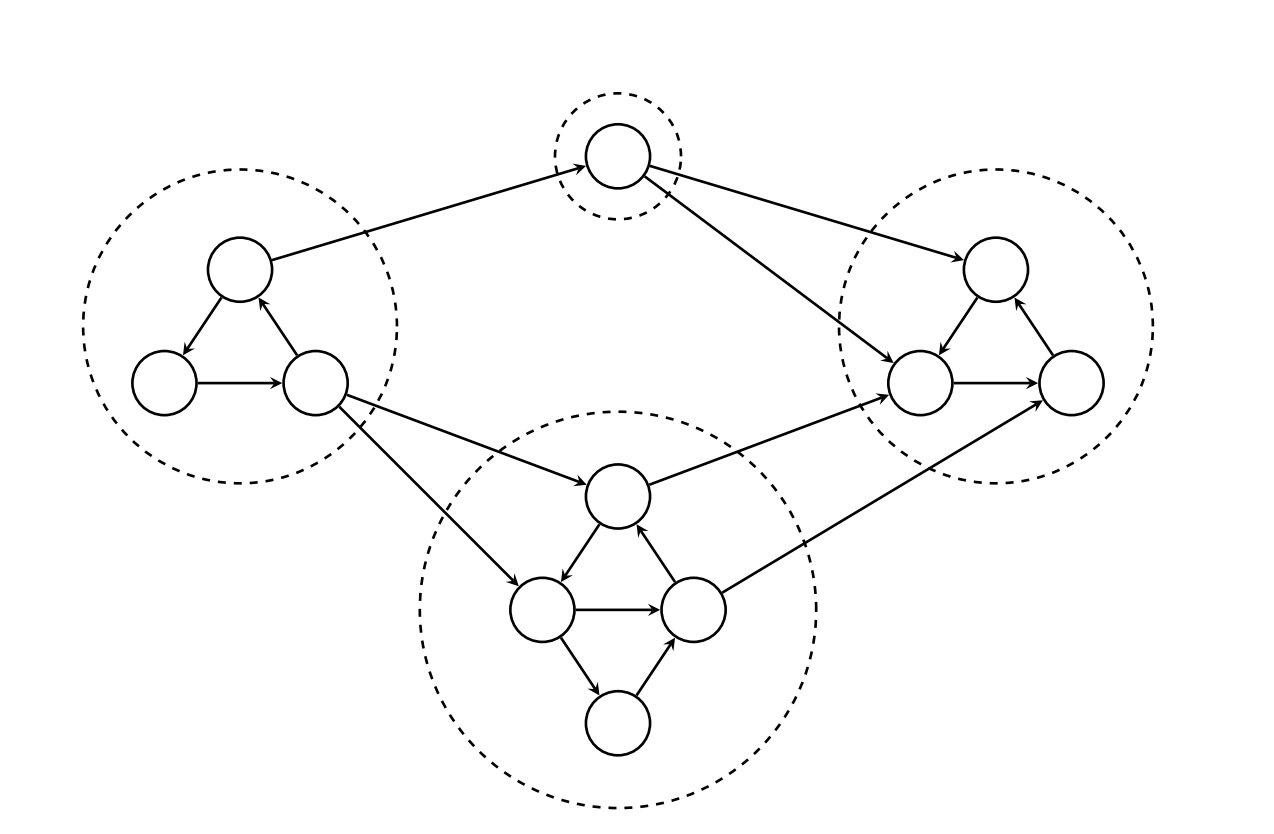
\includegraphics[scale=0.5]{scc_graph.png}
\caption{The strongly connected components of a directed graph}
\label{fig:scc_graph}
\end{figure}


\begin{figure}[ht!]
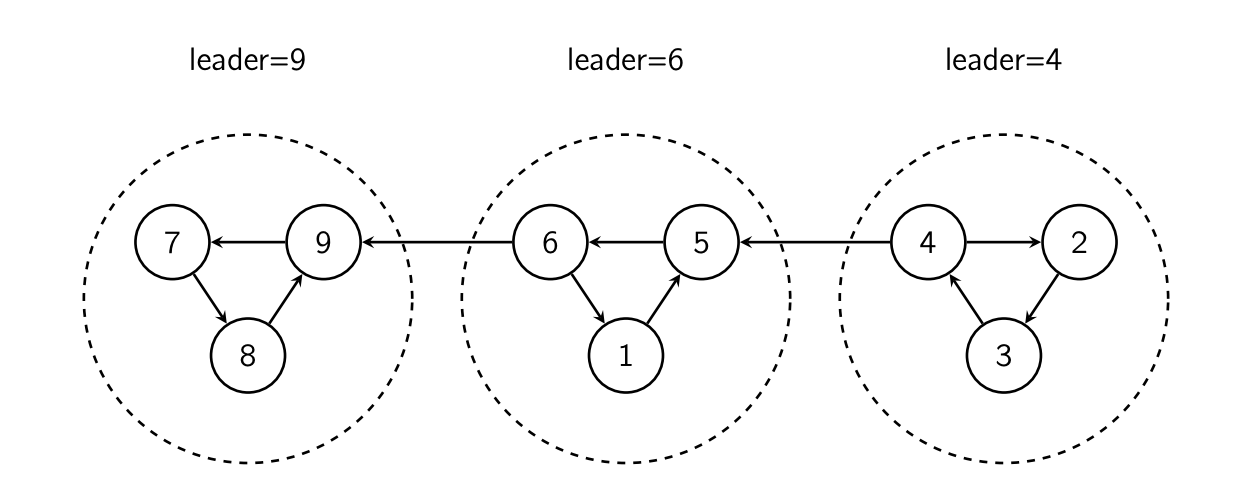
\includegraphics[scale=0.8]{scc_alg.png}
\caption{Example execution of the strongly connected components algorithm. Nodes are labeled by their finishing times and their leaders are shown.}
\label{fig:scc_alg}
\end{figure}

\subsection{The Acyclic Meta-Graph of SCCs} 
First, observe that the strongly connected components of a directed graph form an acyclic ``meta-graph'', where the meta-nodes correspond to the SCCs $C_1, \cdots , C_k$ , and there is an arc $C_h \to C_{\ell}$ with $h \neq \ell$ if and only if there is at least one arc $(i, j)$ in $G$ with $i \in C_h$ and $j \in C_{\ell}$. This directed graph must be acyclic: since within a SCC you can get from anywhere to anywhere else on a directed path, in a purported directed cycle of SCCs you can get from every node in a constituent SCC to every other node of every other SCC in the cycle. Thus the purported cycle of SCCs is actually just a single SCC. Summarizing, every directed graph has a useful ``two-tier'' structure: zooming out, one sees a DAG (Directed Acyclic Graph) on the SCCs of the graph; zooming in on a particular SCC exposes its finer-grained structure. For example, the meta-graphs corresponding to the directed graphs in Figs. \ref{fig:scc_graph} and \ref{fig:scc_alg} are shown in Fig. \ref{fig:meta_graph_scc}.

\begin{figure}
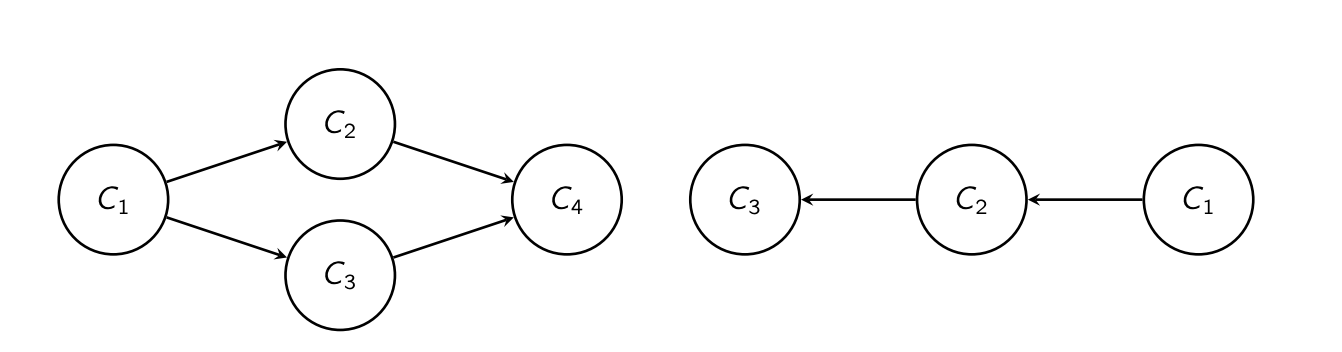
\includegraphics[scale=0.8]{meta_graph_scc.png}
\caption{The DAGs of the SCCs of the graphs in Figs. \ref{fig:scc_graph} and \ref{fig:scc_alg}.}
\label{fig:meta_graph_scc}
\end{figure}

\section{Proof of Correctness}
\subsection{The Key Lemma}
Correctness of the algorithm hinges on the following key lemma.

\begin{lemma} 
Consider two ``adjacent'' strongly connected components of a graph $G$: components $C_1$ and $C_2$ such that there is an arc $(i, j)$ of $G$ with $i \in C_1$ and $j \in C_2$. Let $ f (v )$ denote the finishing time of vertex $v$ in some execution of DFS-Loop on the reversed graph $G^{\text{rev}}$. Then
$$
\max_{v\in C_1} f(v) < \max_{v\in C_2}f(v)
$$
\end{lemma}

\begin{proof} 
Consider two adjacent SCCs $C_1$ and $C_2$, as they appear in the reversed graph $G^{\text{rev}}$ - where there is an arc $(j, i)$, with $j \in C_2$ and $i \in C_1$ (Fig. \ref{fig:scc_proof}). Because the equivalence relation defining the SCCs is symmetric, G and $G^{\text{rev}}$ have the same SCCs; thus $C_1$ and $C_2$ are also SCCs of $G^{\text{rev}}$. Let $v$ denote the first vertex of $C_1 \cup C_2$ visited by DFS-Loop in $G^{\text{rev}}$. There are now two cases. 

First, suppose that $v \in C_1$ (Fig. \ref{fig:scc_proof}). Since there is no non-trivial cycle of SCCs (Section 4.1), there is no directed path from $v$ to $C_2$ in $G^{\text{rev}}$. Since DFS discovers everything reachable and nothing more, it will finish exploring all vertices in $C_1$ without reaching any vertices in $C_2.$ Thus, every finishing time in $C_1$ will be smaller that every finishing time in $C_2$, and this is even stronger than the assertion of the lemma. (Cf., the left and middle SCCs in Fig. \ref{fig:scc_alg}.) Second, suppose that $v \in C_2$ (Fig. \ref{fig:scc_proof}). Since DFS discovers everything reachable and nothing more, the call to DFS at $v$ will finish exploring all of the vertices in $C_1 \cup C_2$ before ending. Thus, the finishing time of $v$ is the largest amongst vertices in $C_1 \cup C_2$, and in particular is larger than all finishing times in $C_1$. (Cf., the middle and right SCCs in Fig. \ref{fig:scc_alg}.)

This completes the proof.
\end{proof}

\begin{figure}
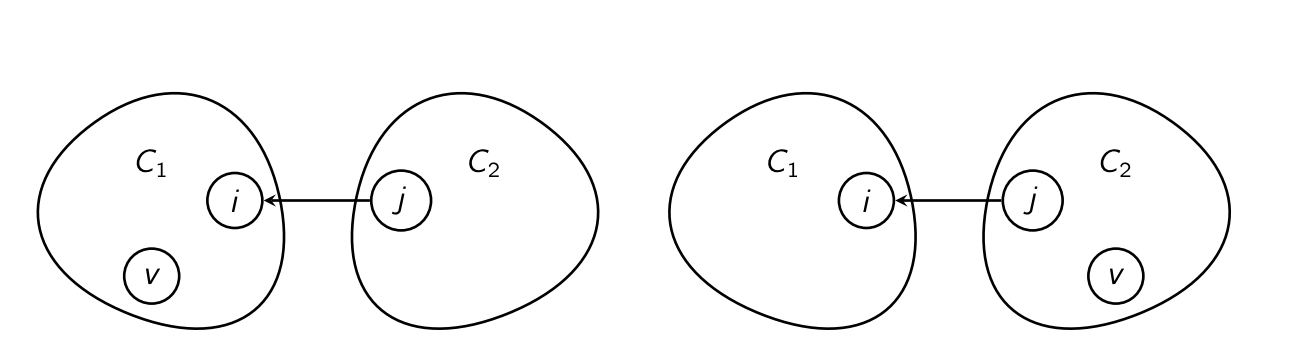
\includegraphics[scale=0.8]{scc_proof.png}
\caption{Proof of key lemma. Vertex $v$ is the first in$ C_1 \cup C_2$ visited during the execution of DFS-Loop on $G^{\text{rev}}$. On the left, all $f$-values in $C_1$ smaller than in $C_2$. On the right: $v$ has the largest $f$-value in $C_1 \cup C_2$.}
\label{fig:scc_proof}
\end{figure}

\subsection{The Final Argument} 

The Key Lemma says that traversing an arc from one SCC to another (in the original, unreversed graph) strictly increases the maximum $f$-value of the current SCC. For example, if $f_i$ denotes the largest $f$-value of a vertex in $C_i$ in Fig. \ref{fig:meta_graph_scc}, then we must have $f_1 < f_2, f_3 < f_4$. Intuitively, when DFS-Loop is invoked on $G$, processing vertices in decreasing order of finishing times, the successive calls to DFS peel off the SCCs of the graph one at a time, like layers of an onion. 

We now formally prove correctness of our algorithm for computing strongly connected components. Consider the execution of DFS-Loop on $G$. We claim that whenever DFS is called on a vertex $v$, the vertices explored - and assigned a common leader - by this call are precisely those in $v$'s SCC in $G$. Since DFS-Loop eventually explores every vertex, this claim implies that the SCCs of $G$ are precisely the groups of vertices that are assigned a common leader. 

We proceed by induction. Let $S$ denote the vertices already explored by previous calls to DFS (initially empty). Inductively, the set $S$ is the union of zero or more SCCs of G. Suppose DFS is called on a vertex $v$ and let $C$ denote $v$'s SCC in $G$. Since the SCCs of a graph are disjoint, $S$ is the union of SCCs of G, and $v \notin S$, no vertices of $C$ lie in $S$. Thus, this call to DFS will explore, at the least, all vertices of $C$. By the Key Lemma, every outgoing arc $(i, j)$ from $C$ leads to some SCC $C'$ that contains a vertex w with a finishing time larger than $f (v)$. Since vertices are processed in decreasing order of finishing time, $w$ has already been explored and belongs to $S$; since $S$ is the union of SCCs, it must contain all of $C'$ . Summarizing, every outgoing arc from $C$ leads directly to a vertex that has already been explored. Thus this call to DFS explores the vertices of $C$ and nothing else. This completes the inductive step and
the proof of correctness.


\section{Dijkstra's Algorithm}

Now we will solve the single source shortest paths problem in graphs with nonnengative
weights using Dijkstra's algorithm. The key idea, that Dijkstra will maintain as an invariant,
is that $\forall t in V$, the algorithm computes an estimate $d[t]$ of the distance of $t$ from the source such that:

\begin{enumerate}
    \item At any point in time, $d[t] \geq d(s, t)$, and
    \item when t is finished, $d[t] = d(s, t)$.
\end{enumerate}


\begin{algorithm}
\caption{Dijkstra($G= (V,E), S$)}
\label{alg:1}
\begin{algorithmic}
\STATE $\forall t \in V, d[t] \gets \infty$ \texttt{// set initial distance estimates}
\STATE $d[s] \gets 0$
\STATE $F \gets \{v \mid \forall v \in V\}$ \texttt{// F is the set of nodes that are yet to achieve final distances estimates}
\STATE $D \gets \emptyset$ \texttt{// D will be the set of nodes that have achieved final distance estimates}
\WHILE{$F \neq \emptyset$}
    \STATE $x \gets$ elements in $F$ with minimum distance estimate
    \FOR{$(x,y) \in E$}
        \STATE $d[y] \gets \min\{d[y], d[x] + w(x,y)\}$ \texttt{// "relax" the estimate of y}
        \STATE \texttt{// to maintain paths: if} $d[y]$ \texttt{changes, then } $\pi(y) \gets x$
    \ENDFOR
    \STATE $F \gets F \setminus \{x\}$
    \STATE $D \gets D \cup \{x\}$
\ENDWHILE
\end{algorithmic}
\end{algorithm}

\begin{claim}[For every $u$, at any point of time $d(u) \geq d(s, u)$.]
\vspace{1em}
A formal proof of this claim proceeds by induction. In particular, one shows that at any point in time, if $d[u] < \infty$, then $d[u]$ is the weight of some path from $s$ to $t$. Thus at any point $d[u]$ is at least the weight of the shortest path, and hence $d[u] \geq d(s, u)$. As a base case, we know that $d[s] = 0 = d(s, s)$ and all other distance estimates are $+\infty$, so we know that the claim holds initially. Now, when $d[u]$ is changed to $d[x] + w(x, u)$ then (by the induction hypothesis) there is a path from $s$ to $x$ of weight $d[x]$ and an edge $(x, u)$ of weight $w(x, u)$. This means there is a path from $s$ to $u$ of weight $d[u] = d[x] + w(x, u)$. This implies that $d[u]$ is at least the weight of the shortest path $= d(s, u)$, and the induction argument is complete
\end{claim}


\begin{claim}[When node $x$ is placed in $D$, $d(x) = d(s,x)$] 
\vspace{1em}

Notice that proving the above claim is sufficient to prove the correctness of the algorithm since $d[x]$ is never changed again after $x$ is added to $D$: the only way it could be changed is if for some node $y \in F$ , $d[y] + w(y, x) < d[x]$ but this can’t happen since $d[x] \leq d[y ]$ and $w(y, x) \geq 0$ (all edge weights are nonnegative). The assertion $d[x] \leq d[y]$ for all $y \in F$ stays true at all points after $x$ is inserted into D: assume for contradiction that at some point for some $y \in F$ we get $d[y ] < d[x]$ and let $y$ be the first such $y$ . $Before d[y ]$ was updated $d[y' ] \geq d[x]$ for all $y' \in F$ . But then when $d[y ]$ was changed, it was due to some neighbor $y'$ of $y$ in $F$ , but$ d[y' ] \geq d[x]$ and all weights are nonnegative, so we get a contradiction 

We prove this claim by induction on the order of placement of nodes into $D$. For the base case, $s$ is placed into D where $d[s] = d(s, s) = 0$, so initially, the claim holds. 

For the inductive step, we assume that for all nodes $y$ currently in $D$, $d[y ] = d(s, y )$. Let $x$ be the node that currently has the minimum distance estimate in $F$ (this is the node about to be moved from $F$ to $D$). We will show that $d[x] = d(s, x)$ and this will complete the induction. Let $p$ be a shortest path from $s$ to $x$. Suppose $z$ is the node on $p$ closest to $x$ for which $d[z] = d(s, z)$. We know $z$ exists since there is at least one such node, namely $s$, where $d[s] = d(s, s)$. By the choice of $z$, for every node $y$ on $p$ between $z$ (not inclusive) to $x$ (inclusive), $d[y ] > d(s, y )$. Consider the following options for $z$.

\begin{enumerate} 
    \item If $z = x$, then $d[x] = d(s, x)$ and we are done.
    \item Suppose $z \neq x$. Then there is a node $z'$ after $z$ on $p$. (Here it is possible that $z' = x$.) We know that $d[z] = d(s, z) \leq d(s, x) \leq d[x]$. The first $\leq$ inequality holds because subpaths of shortest paths are shortest paths as well, so that the prefix of $p$ from $s$ to $z$ has weight $d(s, z)$. In addition, the weights on edges are non-negative, so that the portion of $ p$ from $z$ to $x$ has a nonnegative weight, and so $d(s, z) \leq d(s, x)$. The subsequent $\leq $ holds by Claim 1. We know that if $d[z] = d[x]$ all of the previous inequalities are equalities and $d[x] = d(s, x)$ and the claim holds. 

    Finally, towards a contradiction, suppose $d[z] < d[x]$. By the choice of $x \in F$ we know $d[x]$ is the minimum distance estimate that was in $F$ . Thus, since $d[z] < d[x]$, we know $z \notin F$ and must be in $D$, the finished set. This means the edges out of $z$, and in particular ($z, z' )$, were already relaxed by our algorithm. But this means that $d[z ' ] \leq d(s, z) + w(z, z' ) = d(s, z' )$, because $z$ is on the shortest path from $s$ to $z '$ , and the distance estimate of $z '$ must be correct. However, this contradicts $z$ being the closest node on $p$ to $x$ meeting the criteria$ d[z] = d(s, z)$. Thus, our initial assumption that $d[z] < d[x]$ must be false and $d[x]$ must equal $d(s, x)$.
\end{enumerate}
\end{claim}
\end{document}